\chapter{Development of Synthetic Smokers: Preliminary Experiments}
\label{ch:synthetic-smoker-preliminary}

The iterative development of MIBot (as described in \Cref{ch:mibot}) required that we extensively test it after every change in its prompt. To automate the testing of some aspects of the chatbot's behaviour, we started the development of ``synthetic smokers''\footnote{It is worth mentioning that we also utilized human role-playing as smokers during our testing of MIBot.}. A synthetic smoker, in the context of this research, is a prompted instance of an LLM tasked to simulate the behaviour, language, and psychological responses of a human smoker engaged in a counselling session.

This chapter details the initial conceptualization and preliminary experiments in the development of these synthetic agents. We begin by defining the theoretical framework for creating realistic agents, followed by our early experiments to control behavioural attributes like verbosity and resistance to quitting. These initial steps highlight the core challenges of attribute installation and validation. In the subsequent chapter, we use a more advanced, data-driven methodology for attribute installation and validation.

\section{Objectives and Overview}
\label{sec:synthetic-smoker-goals}

The overarching goal of developing synthetic smokers is to create realistic and controllable proxies for human participants. This endeavour serves two primary objectives:

\begin{enumerate}
    \item \textbf{Testing Automated Systems:} Synthetic smokers provide a platform for the rapid iterative development and testing of automated counselling chatbots. By simulating interactions, developers may identify weaknesses, refine conversational strategies, and assess potential efficiency without the logistical overhead of recruiting human subjects for every iteration.
    \item \textbf{Training Human Clinicians:} In the role of standardized patients, synthetic smokers can be used to train novice clinicians. They offer a consistent experience and can be programmed to simulate specific challenging scenarios or diverse demographic profiles, which could help trainees receive varied practice opportunities.
\end{enumerate}

The development of a truly representative synthetic smoker poses a scientific challenge. It requires not only the generation of coherent dialogue but the accurate embodiment of specific human attributes ranging from demographics to complex psychological states like resistance to change. Crucially, the validation of these synthetic agents (i.e., proving that they behave realistically according to their installed attributes) is exceptionally difficult, as establishing the \textit{construct validity} of behavioural measurements remains a persistent challenge; that is, it is difficult to ensure that an instrument truly measures the specific psychological attribute it purports to assess \cite{Cronbach1955}.


\section{Goals for a Synthetic Smoker}
\label{sec:synthetic-smoker-ideal}

In an ideal scenario, a synthetic smoker would be indistinguishable from a human participant within the constrained context of a smoking cessation counselling session. This requires the synthetic agent to possess a defined set of attributes and for those attributes to be reliably reflected in its interactions and behaviours.

We conceptualize a synthetic smoker based on a collection of attributes that define a human smoker. These attributes can be broadly categorized as:

\begin{itemize}
    \item \textbf{Demographic:} age, sex, education level, cultural background, etc.
    \item \textbf{Behavioural:} smoking history (e.g., Heaviness of Smoking Index (HSI)), previous quit attempts, verbosity, etc.
    \item \textbf{Psychological:} resistance to change, motivation levels (e.g., operationalized by pre-conversation readiness rulers), underlying values, etc.
\end{itemize}

A successful system (or methodology) for creating synthetic smokers must produce agents that exhibit both high \emph{fidelity} and \emph{representativeness}.

\textbf{Fidelity} refers to the requirement that any attribute installed in the synthetic smoker must be demonstrably evidenced by its language and behaviour. For example, if a synthetic smoker is installed with high resistance, its dialogue should contain more Sustain Talk than Change Talk. The core challenge of this research is to develop methods to install these attributes and subsequently validate that this installation was successful.

\textbf{Representativeness} encompasses two key requirements:

\begin{enumerate}
    \item The system must generate a diverse range of smokers whose attributes mirror the variability of the target real-world population. It must avoid the bias of over-representing a narrow or easily simulated archetype at the expense of mirroring the population's true statistical makeup. This may happen for a variety of reasons. For example, if the system is built on biased data, it may fail to generate a statistically accurate population.

    \item The smokers created by the system should exhibit uniform fidelity, i.e., it should not have performance biases where specific profiles are simulated more accurately than others. A system might, for instance, be highly effective at simulating a 55-year-old, heavily dependent smoker with low motivation to quit, while failing to simulate a 22-year-old ``social smoker'' who is ambivalent about quitting. Representativeness requires that the quality of the simulation remains high across the entire spectrum of generated profiles.
\end{enumerate}



Let the collection of all relevant attributes define an $n$-dimensional \emph{attribute space}, $\mathcal{A}$. A specific smoker's profile, whether human or synthetic, is a vector $\textbf{A}$ within this space.
\[\textbf{A} = (a_1, a_2, \ldots, a_n) \in \mathcal{A}\]

The \emph{observable output space}, $\Gamma$, contains all possible outputs from a counselling session, such as conversation transcripts and survey responses. A specific session's output is an element $\gamma \in \Gamma$.
\[\gamma = \{\text{Transcript}, \text{Survey Responses}, \ldots\}\]

Human behaviour is not deterministic; a human $H$ with a given attribute vector $\textbf{A}_H$ will not produce the exact same output in every session. Instead, their behaviour is better modelled as a sample from a conditional probability distribution, $P_H(\gamma | \textbf{A}_H)$. Consequently, a synthetic smoker system, $S$, should not be a deterministic function but a model that approximates this human distribution, $P_S(\gamma | \textbf{A}_S)$. The goal is to ensure that $P_S(\gamma | \textbf{A}) \approx P_H(\gamma | \textbf{A})$.

To assess whether the system has achieved this goal, we must formalize the process of validation. For this, we define a \emph{measurement function}, $M$, that takes an output $\gamma$ and returns an estimated attribute vector $\hat{\textbf{A}}$.

\[M: \Gamma \rightarrow \mathcal{A}, \quad \text{where} \quad \hat{\textbf{A}} = M(\gamma)\]

For example, $M$ could be a set of classifiers and analytical tools that read a transcript and analyse post-conversation changes in behaviour to estimate the speaker's resistance, motivation, smoking history, etc., and produce $\hat{\textbf{A}}$. The measurement function $M$ is an imperfect proxy, as inferring latent constructs from observable behaviour is a persistent challenge in psychometric theory \cite{loevinger1957objective, borsboom2004concept}.

\subsection{Defining Fidelity}
Fidelity measures how accurately the observable outputs of a synthetic smoker reflect its assigned attributes. High fidelity is achieved when the attributes measured from the output, $\hat{\textbf{A}}_S = M(\gamma_S)$, are close to the input attributes, $\textbf{A}_S$. We quantify this correspondence using a distance metric, $d(\textbf{A}_S, \hat{\textbf{A}}_S)$, in the attribute space.

Given the stochastic nature of the generative system, a single instance is insufficient for evaluation. We therefore define the fidelity for a profile $\textbf{A}_S$ as the \emph{expected distance} between the input and measured attributes over the distribution of all possible outputs.
\[\mathcal{F}(\textbf{A}_S) = \mathbb{E}_{\gamma_S \sim P_S(\gamma | \textbf{A}_S)}[d(\textbf{A}_S, M(\gamma_S))]\]
A lower value of $\mathcal{F}(\textbf{A}_S)$ indicates higher fidelity. The objective of the system, then, is to minimize this value across all possible profiles.

In practice, one may not need $M$ to calculate the fidelity, nor is it necessary to recover the full attribute vector $\textbf{A}$. Instead, a more pragmatic approach is to validate individual attributes by demonstrating a strong correlation between their installed values and corresponding, measurable features in the output $\gamma$. For example, to validate the ``resistance to change'' attribute, one can measure a proxy like the percentage Change Talk (\%CT) in the transcript. Evidence of fidelity would be a strong, negative correlation between the installed resistance level and the observed Change Talk across a cohort of synthetic agents. This correlation-based method is more feasible than developing a comprehensive measurement function $M$.

\subsection{Defining Representativeness}

Representativeness ($\mathcal{R}$) ensures that the synthetic population is both a statistically accurate and a consistently well-simulated reflection of the real-world population. It comprises two distinct components.

\subsubsection{Distributional Representativeness}

The first requirement, which we term \textbf{distributional representativeness} ($\mathcal{R}_{dist}$), is that the statistical makeup of the generated synthetic smokers matches that of the target human population. Let $P_H(\textbf{A})$ be the true probability distribution of attribute vectors in the target population. If we generate synthetic agents using a distribution $P_S(\textbf{A})$, this component is high when $P_S(\textbf{A})$ is close to $P_H(\textbf{A})$. We can measure this similarity using the \emph{Kullback-Leibler (KL) Divergence}:
\[\mathcal{R}_{dist} = D_{KL}(P_H(\textbf{A}) \,||\, P_S(\textbf{A})) = \sum_{\textbf{A} \in \mathcal{A}} P_H(\textbf{A}) \log\frac{P_H(\textbf{A})}{P_S(\textbf{A})}\]
A system with high distributional representativeness will minimize this divergence, ensuring that the generated population is not biased towards easily simulated archetypes. Alternatively, to assess whether the system's outputs preserve the population's statistical distribution, one can compare the original input distribution, $P_H(\textbf{A})$, to the distribution of attributes measured from the synthetic agent's final output, $P_S(M(\gamma_S))$.

The KL divergence is a measure of the distortion between the intended input attributes and the measured output attributes:
\[\mathcal{R}_{dist-M} = D_{KL}(P_H(\textbf{A}) \,||\, P_S(M(\gamma_S)))\]
\[= \sum_{\textbf{A} \in \mathcal{A}} P_H(\textbf{A}) \log\frac{P_H(\textbf{A})}{P_S(M(\gamma_S)=\textbf{A})}\]
Here, $P_S(M(\gamma_S)=\textbf{A})$ is the probability that the measured attributes from a synthetic agent's output $\gamma_S$ will equal the vector $\textbf{A}$, when the agent's input profile was drawn from the true human distribution $P_H(\textbf{A})$.

In practice, this is calculated by comparing the empirical distribution of a sample of human attribute vectors $\{\textbf{A}_i\}$ against the distribution of their corresponding measured outputs $\{\hat{\textbf{A}}_i = M(\gamma_i)\}$. This calculation assumes that $M$ faithfully extracts the attributes from $\gamma$, which is not guaranteed. Therefore, a high KL divergence introduces an ambiguity: it may be due to the system's inadequacy in installing $\textbf{A}$, or it could be due to $M$ failing to recover $\textbf{A}$ from $\gamma$.


\subsubsection{Uniform Fidelity}
\label{uniform-fidelity}

The second requirement, \textbf{uniform fidelity} ($\mathcal{R}_{unif}$), stipulates that the simulation quality should be consistent across all types of smoker profiles. The fidelity score, $\mathcal{F}(\textbf{A})$, should not be systematically better for some profiles than for others. We can measure this by calculating the \textit{variance of the fidelity score} across the distribution of real-world smokers, $P_H(\textbf{A})$:
\[\mathcal{R}_{unif} = \text{Var}_{\textbf{A} \sim P_H(\textbf{A})}[\mathcal{F}(\textbf{A})] = \mathbb{E}_{\textbf{A} \sim P_H(\textbf{A})} [(\mathcal{F}(\textbf{A}) - \bar{\mathcal{F}})^2]\]
where $\bar{\mathcal{F}}$ is the mean fidelity across the population. A system that achieves high uniform fidelity will have a value of $\mathcal{R}_{unif}$ close to zero, indicating that its performance is reliable and unbiased across the full spectrum of human smokers. In practice, it is sufficient to calculate fidelity stratified by different relevant attributes (e.g., age groups, sex, ethnicity, etc.) and investigate if a certain group of synthetic agents has low fidelity.


\section{Development of Synthetic Smokers}
We began our development of synthetic smokers by prompting an LLM and providing instructions on how to behave like a smoker in a clinical setting. As we evaluated our synthetic smokers, both our approaches to installation and validation evolved and informed each other. In the following sections, we describe our methodology for creating synthetic smokers along with their validation.


\subsection{The Baseline Synthetic Smoker}
\label{sec:synthetic-smoker-baseline}
The goal of the baseline synthetic smoker was to create a conversational partner that could interact with MIBot prototypes, allowing the researchers to test conversational flow and MI adherence of MIBot in a controlled environment.


\subsubsection{Methodology}
We began with a minimal prompt instructing an LLM (initially GPT-4 Turbo) to adopt the persona of a smoker engaging in a counselling session. The prompt was kept minimal and did not provide a \emph{backstory} or specific behavioural constraints.

\begin{verbatim}
 You are a human smoker engaged in a private thirty-minute session
 with a counsellor. This is your first time talking to a therapist
 about your smoking habits... Respond to the counsellor's inquiries
 as accurately as possible...
\end{verbatim}

Since we did not install any attributes to this baseline, we were mainly looking for how it conversed with MIBot and whether it had some default attributes. We generated a small number ($N=5$) of conversations between this baseline synthetic smoker and an early version of the MIBot counsellor. The validation method at this stage was qualitative human inspection by the research team, including expert MI clinicians.

\subsubsection{Observations}
The transcript of the conversation between MIBot and the baseline synthetic smoker revealed two significant issues that made the synthetic smoker sound ``unnatural'' or atypical of a human smoker:

\begin{enumerate}
    \item Excessive Verbosity: The synthetic smoker tended to produce long, elaborate responses. This felt unnatural and resembled written prose more than spontaneous dialogue.
    \item High Agreeableness (Low Resistance): The baseline agent was overly agreeable and eager to change. This failed to simulate the ambivalence characteristic of many smokers seeking cessation support (as discussed in \Cref{ch:background}).
\end{enumerate}

These observations highlighted the necessity of explicitly controlling these attributes.

\subsection{Controlling Verbosity}
\label{sec:synthetic-smoker-verbosity}

To address the issue of excessive verbosity, we undertook a prompt engineering effort to constrain the synthetic smoker's utterance length and style.

\subsubsection{Methodology}
We modified the prompt to encourage a more natural, concise conversational style. Key additions to the prompt included:

\begin{itemize}
    \item Stylistic Guidance: Instructions such as ``Imagine you're texting a friend. Keep it casual...'' and encouraging the use of emojis.
    \item Instructions to be Concise: Directives like ``speak with more clarity rather than exhaustive detail.''
    \item Explicit Constraints: Hard constraints such as ``Number of sentences in your response must be between 1 and 4.''
\end{itemize}

\subsubsection{Validation}
To validate the effectiveness of these changes, we generated a new set of conversations ($n=5$) using the modified prompt (``Fixed Verbosity'') and with GPT-4 Turbo (temperature $=1.0$) and compared them against the baseline prompt (``Default Verbosity''). We also compared these results against human-human MI conversations from the High-Quality and Low-Quality Counselling (HLQC) datasets~\citep{perez-rosas-etal-2019-makes}.

\subsubsection{Results}
The prompt modifications significantly reduced the verbosity of the synthetic smoker. \Cref{fig:verbosity-comparison} illustrates the distribution of volley lengths (in terms of number of words).


\begin{figure}[htpb]
    \centering
    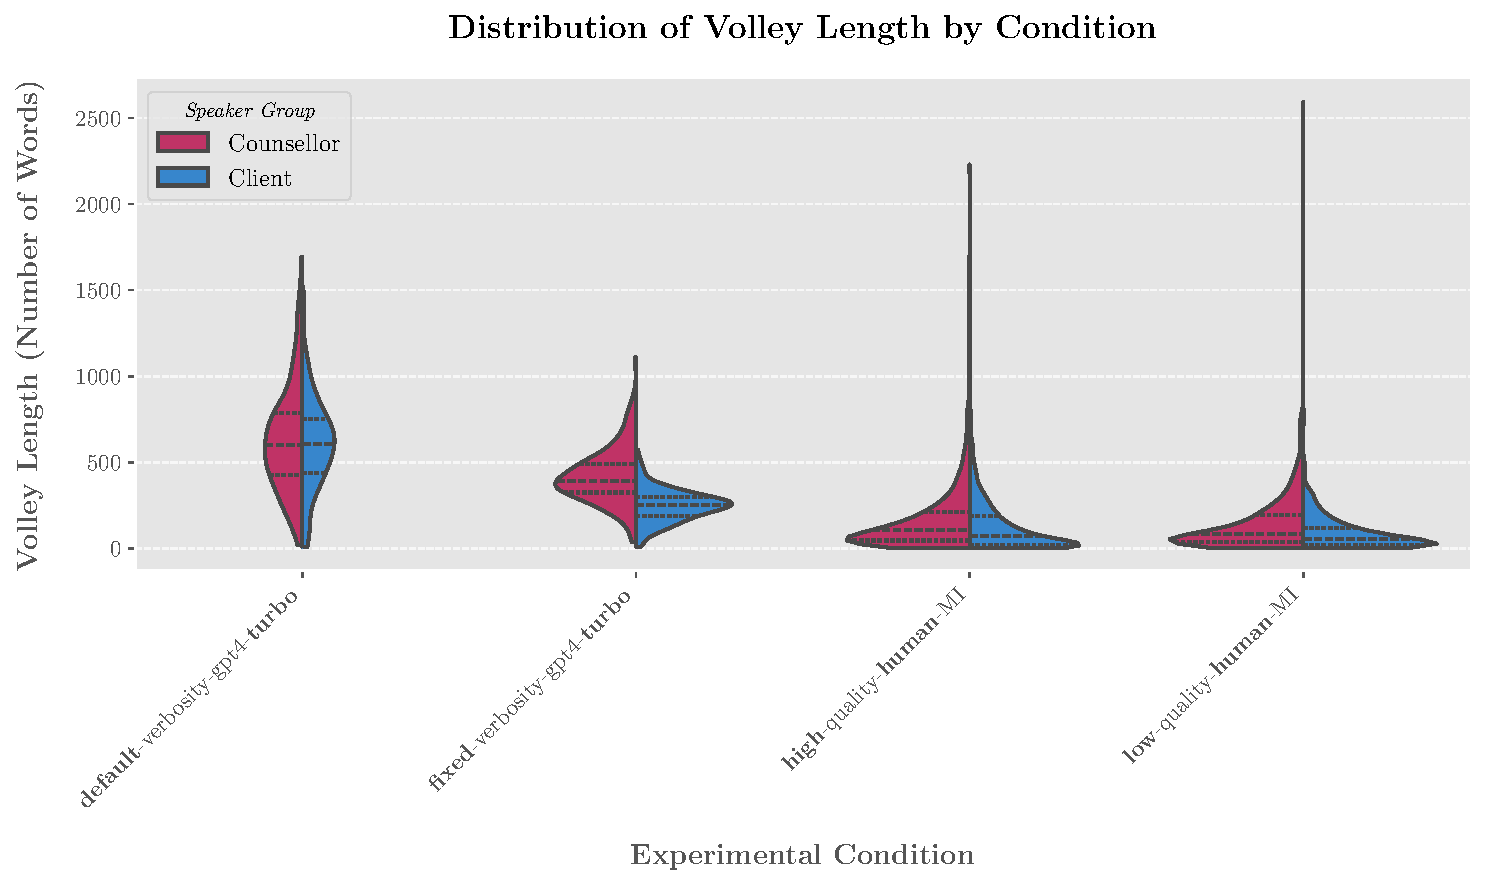
\includegraphics[width=0.9\textwidth]{fig/utterance_length_violin_plot.pdf}
    \caption[Distribution of volley length for default and fixed-verbosity synthetic smokers]{Comparison of utterance length distributions for default and fixed-verbosity synthetic smokers. The fixed-verbosity prompt successfully reduced the synthetic smoker's utterance length to better align with humans (\texttt{high-quality-human-MI}).}
    \label{fig:verbosity-comparison}
\end{figure}

\begin{table}[ht]
\centering

\begin{tabular}{lrr}
\toprule
{} &  \textbf{Mean} &  \textbf{Standard} \\
\textbf{Category}                   &                        &           {Deviation}          \\
\midrule
Default Verbosity (GPT-4 Turbo) &                  618.9 &               296.3 \\
Fixed Verbosity (GPT-4 Turbo)   &                  337.8 &               157.9 \\
High-Quality Human Counselling             &                  147.0 &               172.9 \\
Low-Quality Human Counselling            &                  118.2 &               158.0 \\
\bottomrule
\end{tabular}
\caption{Statistics on Volley Length for Low- and High-Verbosity Synthetic Smokers.}
\label{tab:utterance_stats}
\end{table}

The default verbosity condition showed a wide distribution with a high median utterance length. The fixed-verbosity synthetic smokers successfully matched the distribution with humans from the HQLC dataset. \Cref{tab:utterance_stats} provides detailed statistics on the volley lengths.

Interestingly, we observed that the counsellor bot reciprocated the client's verbosity. When the synthetic smoker spoke less, the counsellor bot also reduced its utterance length. We also verified that these prompt modifications were robust and transferable across different LLMs (GPT-4 Turbo and GPT-4 Omni).

\subsection{Installing Resistance}
\label{sec:synthetic-smoker-resistance}

Addressing the baseline smoker's high agreeableness was crucial, as addressing resistance to change is a crucial MI skill.

\subsubsection{Methodology}
We hypothesized that resistance could be installed by providing the LLM with detailed backstories emphasizing different motivations and experiences. We created two distinct personas:

\begin{itemize}
    \item High Resistance Persona: The backstory emphasized severe life stressors, repeated failed quit attempts, skepticism towards therapy, and a strong belief that it was not the right time to quit.
    \item Low Resistance Persona: The backstory described recent health concerns prompting contemplation, and an open, albeit skeptical, attitude towards change.
\end{itemize}

Using modified prompts and GPT-4 Turbo (temperature=1.0), we generated conversations (N=10 per persona) between synthetic smokers and MIBot. We employed two distinct methods to validate the installation. We also prompted these synthetic smokers to fill the readiness rulers before, after, and a week after the conversation. We did so by prompting the synthetic smoker with the exact questions from the readiness rulers survey. Before reporting the numbers, we asked them to think and provide reasons for the numerical rating they chose before outputting the rating---a technique known as chain-of-thought prompting.

\subsubsection{Validation}

\begin{enumerate}
    \item Linguistic Evidence (Change vs. Sustain Talk): We analysed the transcripts to measure the proportion of Change Talk (CT) and Sustain Talk (ST).


    \item Behavioural Evidence (Self-Reported Readiness): We further validated the installation by asking the synthetic smokers to complete the Readiness Ruler survey (Importance, Confidence, and Readiness; 0--10 scale) before, immediately after, and \emph{simulated} one week after the conversation.

\end{enumerate}






\subsubsection{Results} 



\begin{table}[ht!]
\centering
\begin{tabular}{@{}llll@{}}
\toprule
\textbf{Persona} & \textbf{Change Talk (\%)} & \textbf{Sustain Talk (\%)} & \textbf{Neutral (\%)} \\ \midrule
High Resistance & 31 & 44 & 25 \\
Low Resistance & 61 & 9 & 30 \\ \bottomrule
\end{tabular}
\caption{\% Change, sustain, and neutral talk for high- and low-resistance synthetic smokers.}
\label{tab:resistance-ct-st}
\end{table}

\begin{table}[ht!]
  \centering
  \small
  \renewcommand{\arraystretch}{1.2} % Increased spacing slightly for readability
  \resizebox{\linewidth}{!}{\begin{tabular*}{\linewidth}{@{\extracolsep{\fill}}llcccc@{}}
    \toprule
    \textbf{} & \textbf{} & \textbf{Pre-} & \textbf{Post-} & \textbf{1-week} & \textbf{} \\
       
        \textbf{Client} & & \textbf{conversation} & \textbf{conversation} & \textbf{Follow-up} & \textbf{Change from} \\
        
    \textbf{Resistance}  &  \textbf{Variable} & \textbf{mean (SD)} & \textbf{mean (SD)} & \textbf{mean (SD)} & \textbf{Baseline} \\
    \midrule
    \multirow{3}{*}{Low} & Importance & 4.6 (0.5) & 5.4 (0.9) & 6.6 (0.5) & 2.0 (0.7) \\
    & Confidence & 2.6 (0.5) & 4.2 (1.1) & 4.8 (0.4) & 2.2 (0.4) \\
    & Readiness  & 3.2 (1.1) & 5.2 (1.1) & 5.4 (0.9) & 2.2 (1.9) \\
    \midrule
    \multirow{3}{*}{High} & Importance & 2.0 (0.0) & 4.0 (0.7) & 4.6 (1.1) & 2.6 (1.1) \\
    & Confidence & 1.0 (0.0) & 2.0 (0.0) & 2.6 (0.9) & 1.6 (0.9) \\
    & Readiness  & 0.6 (0.5) & 2.6 (0.5) & 3.4 (1.1) & 2.8 (1.1) \\
    \bottomrule
  \end{tabular*}}
  \caption[Readiness rulers reported by high- and low-resistance synthetic smokers]{Longitudinal changes in self-reported scores (0--10 scale) for importance, confidence, and readiness, stratified by client (synthetic smoker) resistance level. Values were assessed at baseline (pre-conversation), immediately post-conversation, and at 1-week follow-up. Change scores represent the difference between baseline and 1-week follow-up. SD = standard deviation.}
  \label{tab:resistance-readiness-rulers}
\end{table}


The analysis confirmed a clear distinction between the two personas (\Cref{tab:resistance-ct-st}). The High Resistance smoker used significantly more Sustain Talk (44\% vs. 9\%) and less Change Talk (31\% vs. 61\%) than the Low Resistance smoker.


The readiness ruler scores demonstrated that the synthetic smokers provided responses consistent with their installed resistance levels (\Cref{tab:resistance-readiness-rulers}). The ``high-resistance'' synthetic smokers reported lower mean scores on all three dimensions of the readiness rulers. Interestingly, their week-later change in confidence was lower than ``low-resistance'' smokers by 0.8 points, while the change in importance and readiness was slightly higher.




This experiment also provided us with our first evidence that LLM-based synthetic smokers could self-report their smoking behaviours numerically and that the numbers were consistent with the installed attributes. We did notice, however, that the variability of scores was much lower---especially for pre-conversation readiness numbers---as the only source of stochasticity among these agents was the decoding temperature of the underlying LLM.



\section{Conclusion}
\label{sec:prelim-conclusion}

The preliminary experiments detailed in this chapter successfully established a foundation for creating synthetic smokers. We demonstrated that through prompt engineering, it is possible to control basic conversational attributes such as \textbf{verbosity} and install psychological constructs like \textbf{resistance}. Through our validation methods, which included linguistic analysis (\%CT) and behavioural self-reports (readiness rulers), we confirmed that these installed attributes were reflected in the agents' outputs.

These initial studies, however, also revealed significant limitations. The personas were created with arbitrary backstories, which made it difficult to assess the \textbf{representativeness} of our synthetic population against a real-world target demographic. Validating the \textbf{fidelity} of these agents remained a challenge without a direct human counterpart for comparison. To address these issues and move towards a more rigorous validation framework, we needed a data-driven approach. The next chapter introduces the ``doppelgänger'' methodology, a technique designed to create synthetic twins of actual human participants, allowing for a direct and robust assessment of our system's fidelity and representativeness.